\documentclass[a4paper, 12pt]{article}

\usepackage[utf8]{inputenc}
\usepackage{amssymb}
\usepackage{amsmath}
\usepackage{tikz}
\usetikzlibrary{positioning,matrix}

\begin{document}

% https://data-mining.philippe-fournier-viger.com/how-to-draw-an-fp-tree-with-latex-and-tikz/

\begin{figure}
  \centering
  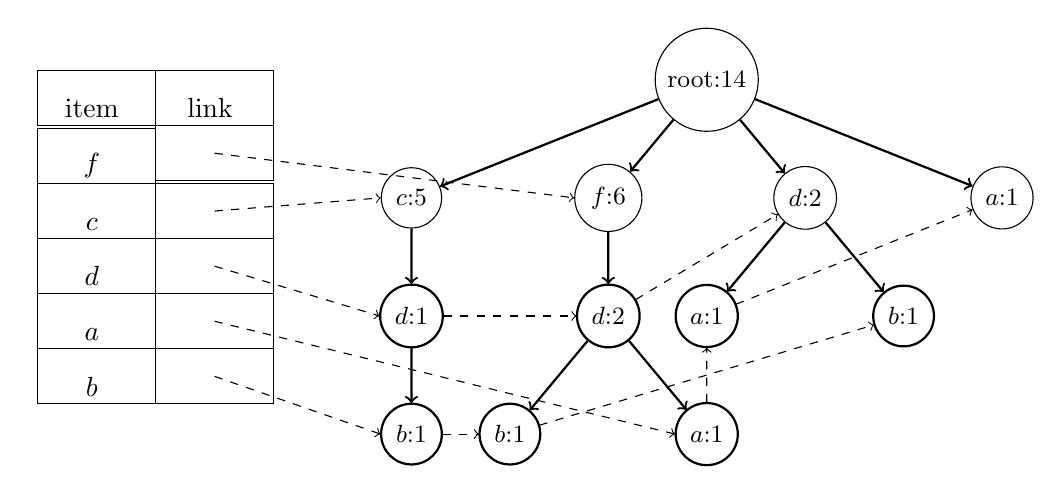
\begin{tikzpicture}
    %%%%% THE TREE
    \begin{scope}[->,font=\small,draw,circle, every node/.style={fill=white!10,shape=circle,draw},
        edge from parent/.style={black,thick,draw},
        level 1/.style={sibling distance=2.5cm},
        level 2/.style={sibling distance=2.5cm}]
      \node (TREE) {root:14}
      child {node {$c$:5}
          child {node {$d$:1}
              child {node {$b$:1}}}}
      child {node {$f$:6}
          child {node {$d$:2}
              child {node {$b$:1}}
              child {node {$a$:1}}}}
      child {node {$d$:2}
          child {node {$a$:1}}
          child {node {$b$:1}}}
      child {node {$a$:1}};
      % Node links within the tree
      \draw[->, dashed] (TREE-1-1) -- (TREE-2-1);
      \draw[->, dashed] (TREE-2-1) -- (TREE-3);
      \draw[->, dashed] (TREE-1-1-1) -- (TREE-2-1-1);
      \draw[->, dashed] (TREE-2-1-1) -- (TREE-3-2);
      \draw[->, dashed] (TREE-2-1-2) -- (TREE-3-1);
      \draw[->, dashed] (TREE-3-1) -- (TREE-4);
    \end{scope}
    %%%%% THE TABLE
    \begin{scope}[xshift=-7cm,yshift=-2cm,every tree node/.style={shape=rectangle,draw}]
      \matrix (TABLE) [matrix of nodes,
        row sep=-\pgflinewidth, column sep=-\pgflinewidth,
        nodes={draw, text height=5mm,
            align=center, minimum width=15mm, inner sep=0mm, minimum height=7mm}]{
        item & link \\
        $f$  & ~    \\
        $c$  & ~    \\
        $d$  & ~    \\
        $a$  & ~    \\
        $b$  & ~    \\
      };
    \end{scope}
    %%%% LINKS FROM THE TABLE TO THE TREE
    \draw[->, dashed] (TABLE-2-2.center) to (TREE-2.west);
    \draw[->, dashed] (TABLE-3-2.center) to (TREE-1.west);
    \draw[->, dashed] (TABLE-4-2.center) to (TREE-1-1.west);
    \draw[->, dashed] (TABLE-5-2.center) to (TREE-2-1-2.west);
    \draw[->, dashed] (TABLE-6-2.center) to (TREE-1-1-1.west);
  \end{tikzpicture}
  \caption{FP-tree projected on $\{\}$}
  \label{fig:FP-tree}
\end{figure}

\begin{figure}
  \centering
  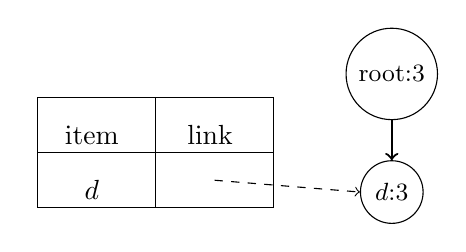
\begin{tikzpicture}
    %%%%% THE TREE
    \begin{scope}[->,font=\small,draw,circle, every node/.style={fill=white!10,shape=circle,draw},
        edge from parent/.style={black,thick,draw},
        level 1/.style={sibling distance=2.5cm},
        level 2/.style={sibling distance=2.5cm}]
      \node (TREE) {root:3}
      child {node {$d$:3}};
      % Node links within the tree
    \end{scope}
    %%%%% THE TABLE
    \begin{scope}[xshift=-3cm,yshift=-1cm,every tree node/.style={shape=rectangle,draw}]
      \matrix (TABLE) [matrix of nodes,
        row sep=-\pgflinewidth, column sep=-\pgflinewidth,
        nodes={draw, text height=5mm,
            align=center, minimum width=15mm, inner sep=0mm, minimum height=7mm}]{
        item & link \\
        $d$  & ~    \\
      };
    \end{scope}
    %%%% LINKS FROM THE TABLE TO THE TREE
    \draw[->, dashed] (TABLE-2-2.center) to (TREE-1.west);
  \end{tikzpicture}
  \caption{FP-tree projected on $\{b\}$}
  \label{fig:FP-tree-b}
\end{figure}

\begin{figure}
  \centering
  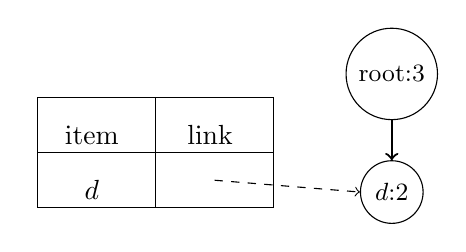
\begin{tikzpicture}
    %%%%% THE TREE
    \begin{scope}[->,font=\small,draw,circle, every node/.style={fill=white!10,shape=circle,draw},
        edge from parent/.style={black,thick,draw},
        level 1/.style={sibling distance=2.5cm},
        level 2/.style={sibling distance=2.5cm}]
      \node (TREE) {root:3}
      child {node {$d$:2}};
      % Node links within the tree
    \end{scope}
    %%%%% THE TABLE
    \begin{scope}[xshift=-3cm,yshift=-1cm,every tree node/.style={shape=rectangle,draw}]
      \matrix (TABLE) [matrix of nodes,
        row sep=-\pgflinewidth, column sep=-\pgflinewidth,
        nodes={draw, text height=5mm,
            align=center, minimum width=15mm, inner sep=0mm, minimum height=7mm}]{
        item & link \\
        $d$  & ~    \\
      };
    \end{scope}
    %%%% LINKS FROM THE TABLE TO THE TREE
    \draw[->, dashed] (TABLE-2-2.center) to (TREE-1.west);
  \end{tikzpicture}
  \caption{FP-tree projected on $\{a\}$}
  \label{fig:FP-tree-a}
\end{figure}

\begin{figure}
  \centering
  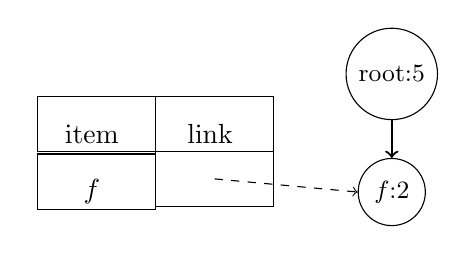
\begin{tikzpicture}
    %%%%% THE TREE
    \begin{scope}[->,font=\small,draw,circle, every node/.style={fill=white!10,shape=circle,draw},
        edge from parent/.style={black,thick,draw},
        level 1/.style={sibling distance=2.5cm},
        level 2/.style={sibling distance=2.5cm}]
      \node (TREE) {root:5}
      child {node {$f$:2}};
      % Node links within the tree
    \end{scope}
    %%%%% THE TABLE
    \begin{scope}[xshift=-3cm,yshift=-1cm,every tree node/.style={shape=rectangle,draw}]
      \matrix (TABLE) [matrix of nodes,
        row sep=-\pgflinewidth, column sep=-\pgflinewidth,
        nodes={draw, text height=5mm,
            align=center, minimum width=15mm, inner sep=0mm, minimum height=7mm}]{
        item & link \\
        $f$  & ~    \\
      };
    \end{scope}
    %%%% LINKS FROM THE TABLE TO THE TREE
    \draw[->, dashed] (TABLE-2-2.center) to (TREE-1.west);
  \end{tikzpicture}
  \caption{FP-tree projected on $\{d\}$}
  \label{fig:FP-tree-d}
\end{figure}

\begin{figure}
  \centering
  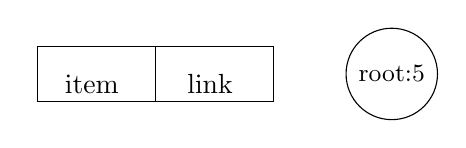
\begin{tikzpicture}
    %%%%% THE TREE
    \begin{scope}[->,font=\small,draw,circle, every node/.style={fill=white!10,shape=circle,draw},
        edge from parent/.style={black,thick,draw},
        level 1/.style={sibling distance=2.5cm},
        level 2/.style={sibling distance=2.5cm}]
      \node (TREE) {root:5};
      % Node links within the tree
    \end{scope}
    %%%%% THE TABLE
    \begin{scope}[xshift=-3cm,yshift=-0cm,every tree node/.style={shape=rectangle,draw}]
      \matrix (TABLE) [matrix of nodes,
        row sep=-\pgflinewidth, column sep=-\pgflinewidth,
        nodes={draw, text height=5mm,
            align=center, minimum width=15mm, inner sep=0mm, minimum height=7mm}]{
        item & link \\
      };
    \end{scope}
    %%%% LINKS FROM THE TABLE TO THE TREE
  \end{tikzpicture}
  \caption{FP-tree projected on $\{c\}$}
  \label{fig:FP-tree-c}
\end{figure}

\begin{figure}
  \centering
  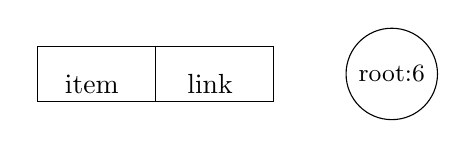
\begin{tikzpicture}
    %%%%% THE TREE
    \begin{scope}[->,font=\small,draw,circle, every node/.style={fill=white!10,shape=circle,draw},
        edge from parent/.style={black,thick,draw},
        level 1/.style={sibling distance=2.5cm},
        level 2/.style={sibling distance=2.5cm}]
      \node (TREE) {root:6};
      % Node links within the tree
    \end{scope}
    %%%%% THE TABLE
    \begin{scope}[xshift=-3cm,yshift=-0cm,every tree node/.style={shape=rectangle,draw}]
      \matrix (TABLE) [matrix of nodes,
        row sep=-\pgflinewidth, column sep=-\pgflinewidth,
        nodes={draw, text height=5mm,
            align=center, minimum width=15mm, inner sep=0mm, minimum height=7mm}]{
        item & link \\
      };
    \end{scope}
    %%%% LINKS FROM THE TABLE TO THE TREE
  \end{tikzpicture}
  \caption{FP-tree projected on $\{f\}$}
  \label{fig:FP-tree-f}
\end{figure}

\end{document}
